%% Преамбула TeX-файла

% 1. Стиль и язык
\documentclass[utf8x]{G7-32} % Стиль (по умолчанию будет 14pt)
\usepackage[T2A]{fontenc}
\usepackage[russian]{babel}
% Остальные стандартные настройки убраны в preamble.inc.tex.
%%==========================================%%
%% Для избежания переносов слов
\usepackage{ragged2e}
\usepackage{microtype}

\justifying
\sloppy
\tolerance=500
\hyphenpenalty=10000
\emergencystretch=3em
%%==========================================%%

% Настройки стиля ГОСТ 7-32
% Для начала определяем, хотим мы или нет, чтобы рисунки и таблицы нумеровались в пределах раздела, или нам нужна сквозная нумерация.
\EqInChapter % формулы будут нумероваться в пределах раздела
\TableInChapter % таблицы будут нумероваться в пределах раздела
\PicInChapter % рисунки будут нумероваться в пределах раздела

% Добавляем гипертекстовое оглавление в PDF
\usepackage[
bookmarks=true, colorlinks=true, unicode=true,
urlcolor=black,linkcolor=black, anchorcolor=black,
citecolor=black, menucolor=black, filecolor=black,
]{hyperref}

%Величина «красной строки»


\usepackage[tableposition=top,singlelinecheck=false]{caption}
%\usepackage{subcaption}

\DeclareCaptionLabelFormat{gostfigure}{Рисунок #2}
\DeclareCaptionLabelFormat{gosttable}{Таблица #2}
\DeclareCaptionLabelSeparator{gost}{~---~}
% Можно разбивать длинные таблицы вручную, оформляя каждую как table. В этом случае для продолжений таблицы нужно создать отдельный стиль заголовка
\DeclareCaptionLabelFormat{continued}{Продолжение таблицы~#2}
\captionsetup*[ContinuedFloat]{labelformat=continued}
\captionsetup{labelsep=gost}
\captionsetup*[figure]{labelformat=gostfigure, justification=centering,font={small, bf}}  % выравнивание по центру
\captionsetup*[table]{hangindent=-10pt, indention=0pt,parindent=0pt,margin=0pt,labelformat=gosttable,justification=raggedright,font={small,it}}
\captionsetup*[lstlisting]{font={small, it}}

% Изменение начертания шрифта --- после чего выглядит таймсоподобно.
% apt-get install scalable-cyrfonts-tex

\IfFileExists{cyrtimes.sty}
    {
        \usepackage{cyrtimespatched}
    }
    {
        % А если Times нету, то будет CM...
    }

\usepackage{graphicx}   % Пакет для включения рисунков
%расположение графики
\graphicspath{{images/}{figures/}{screnshots/}{../images/}}  % папки с картинками

% С такими оно полями оно работает по-умолчанию:
% \RequirePackage[left=20mm,right=10mm,top=20mm,bottom=20mm,headsep=0pt]{geometry}
% Если вас тошнит от поля в 10мм --- увеличивайте до 20-ти, ну и про переплёт не забывайте:
\geometry{right=10mm}
\geometry{left=30mm}


% Пакет Tikz
\usepackage{tikz}
\usetikzlibrary{arrows,positioning,shadows}

% Произвольная нумерация списков.
\usepackage{enumerate}

% ячейки в несколько строчек
\usepackage{multirow}

% itemize внутри tabular
\usepackage{paralist,array}


% Настройки листингов.
% 8 Листинги

\usepackage{listings}

% Значения по умолчанию
\lstset{
  basicstyle= \footnotesize\ttfamily,
  breakatwhitespace=true,% разрыв строк только на whitespacce
  breaklines=true,       % переносить длинные строки
%   captionpos=b,          % подписи снизу -- вроде не надо
  inputencoding=koi8-r,
  numbers=left,          % нумерация слева
  numberstyle=\footnotesize,
  showspaces=false,      % показывать пробелы подчеркиваниями -- идиотизм 70-х годов
  showstringspaces=false,
  showtabs=false,        % и табы тоже
  stepnumber=1,
  tabsize=4,              % кому нужны табы по 8 символов?
  frame=single
}

% Стиль для псевдокода: строчки обычно короткие, поэтому размер шрифта побольше
\lstdefinestyle{pseudocode}{
  basicstyle=\small\ttfamily,
  keywordstyle=\color{black}\bfseries\underbar,
  language=Pseudocode,
  numberstyle=\footnotesize,
  commentstyle=\footnotesize\it\texttt
}

% Стиль для обычного кода: маленький шрифт
\lstdefinestyle{realcode}{
  basicstyle=\scriptsize,
  numberstyle=\footnotesize
}

% Стиль для коротких кусков обычного кода: средний шрифт
\lstdefinestyle{simplecode}{
  basicstyle=\footnotesize,
  numberstyle=\footnotesize
}

% Стиль для BNF
\lstdefinestyle{grammar}{
  basicstyle=\footnotesize,
  numberstyle=\footnotesize,
  stringstyle=\bfseries\ttfamily,
  language=BNF
}

% Определим свой язык для написания псевдокодов на основе Python
\lstdefinelanguage[]{Pseudocode}[]{Python}{
  morekeywords={each,empty,wait,do},% ключевые слова добавлять сюда
  morecomment=[s]{\{}{\}},% комменты {а-ля Pascal} смотрятся нагляднее
  literate=% а сюда добавлять операторы, которые хотите отображать как мат. символы
    {->}{\ensuremath{$\rightarrow$}~}2%
    {<-}{\ensuremath{$\leftarrow$}~}2%
    {:=}{\ensuremath{$\leftarrow$}~}2%
    {<--}{\ensuremath{$\Longleftarrow$}~}2%
}[keywords,comments]

% Свой язык для задания грамматик в BNF
\lstdefinelanguage[]{BNF}[]{}{
  morekeywords={},
  morecomment=[s]{@}{@},
  morestring=[b]",%
  literate=%
    {->}{\ensuremath{$\rightarrow$}~}2%
    {*}{\ensuremath{$^*$}~}2%
    {+}{\ensuremath{$^+$}~}2%
    {|}{\ensuremath{$|$}~}2%
}[keywords,comments,strings]

% Подписи к листингам на русском языке.
\renewcommand\lstlistingname{\cyr\CYRL\cyri\cyrs\cyrt\cyri\cyrn\cyrg}
\renewcommand\lstlistlistingname{\cyr\CYRL\cyri\cyrs\cyrt\cyri\cyrn\cyrg\cyri}


% Полезные макросы листингов.
% Любимые команды
\newcommand{\Code}[1]{\textbf{#1}}


\renewcommand{\rmdefault}{ftm}

\begin{document}

\frontmatter % выключает нумерацию ВСЕГО; здесь начинаются ненумерованные главы: реферат, введение, глоссарий, сокращения и прочее.

% Команды \breakingbeforechapters и \nonbreakingbeforechapters
% управляют разрывом страницы перед главами.
% По-умолчанию страница разрывается.

% \nobreakingbeforechapters
% \breakingbeforechapters

%% Также можно использовать \Referat, как в оригинале
\begin{abstract}
Это пример каркаса расчётно-пояснительной записки, желательный к использованию в РПЗ проекта по курсу РСОИ.

Данный опус, как и более новые версии этого документа, можно взять по адресу (\url{https://github.com/rominf/latex-g7-32}).

Текст в документе носит совершенно абстрактный характер.
\end{abstract}

%%% Local Variables: 
%%% mode: latex
%%% TeX-master: "rpz"
%%% End: 


\tableofcontents

%\Defines % Необходимые определения. Вряд ли понадобться
\begin{description}
\item[Распределённый] Слово, которое нельзя употреблять. Но надо протестировать длинные строки в глоссарии.
\end{description}

%%% Local Variables:
%%% mode: latex
%%% TeX-master: "rpz"
%%% End:

\Abbreviations %% Список обозначений и сокращений в тексте
% по алфавиту от англ к русским
\begin{description}
\item [CDC] Clock domain crossing. Пересечение доменов синхрочастоты
\item [CLI] Command line interface
\item [DDL] Data Definition Language
\item [DML] Data Manipulation Language
\item [CSS] Cascading Style Sheets
\item [HTML] HyperText Markup Language
\item[SQL] Structured query language.
\item[БД] База данных.
\item[ПО] Программное обеспечение.
\item[СУБД] Система управления базами данных.

\end{description}

%%% Local Variables:
%%% mode: latex
%%% TeX-master: "rpz"
%%% End:


\Introduction



Целью работы является построение цифрового устройства ресинхронизации данных. Данное устройство представляет собой FIFO с восьмиразрядным входом и тридцатидвух разрядным выходом. Данные на выход подаются по мере образования во входном буфере не менее 4 8-разрядных слов. Тактовые сигналы входного и выходного каналов независимы, однако тактовая частота для выхода FIFO составляет как минимум  четверть от тактовой частоты входного интерфейса FIFO.


%\begin{itemize}
%\item проанализировать предложенную ;
%\item спроектировать свою, новую всячину;
%\item изготовить всякую всячину;
%\item проверить её работоспособность.
%\end{itemize}
%
%Вот так-то. А этот абзац вставлен для визуальной оценки отступа от перечня до следующего абзаца.

\mainmatter % это включает нумерацию глав и секций в документе ниже

\newcommand{\erassistant}{ErAssistant~}

\chapter{ПРОБЛЕМАТИКА СИНХРОНИЗАЦИИ}

В данном разделе будут рассмотрены проблемы и особенности построение устройств


В этом разделе будут описаны проблемы, возникающие в процессе разработки мультисихронного проекта, то есть устройства, в котором имеют место пересечения клоковых доменов или доменов синхрочастоты (CDC).

\section{Домен синхрочастоты}
Домен синхрочастоты представляет собой ту часть проекта, которая тактируется одной или несколькими синхрочастотами, причем все эти синхрочастоты должны иметь постоянные сдвиги фазы. Если в какой-либо части проекта имеется синхрочастота или инвертированная синхрочастота, или синхрочастота, полученная из исходной путем деления на 2, то такая часть проекта считается клоковым доменом с одной синхрочастотой. Если же домены имеют синхрочастоты с переменной фазой и соотношениями времени, то такие домены считают доменами с различными синхрочастотами. 

На Рисунке \ref{fig:clock-domain} показано, что проект имеет единственный домен синхрочастоты, потому что синхрочастота divClk --- есть деленная на два частота генератора синхронизации Clk.

\begin{figure}[h!]
	\centering
	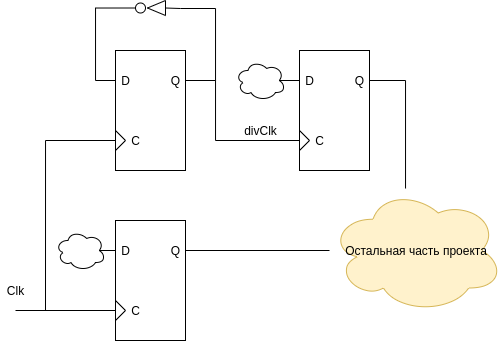
\includegraphics[width=0.5\linewidth]{course-scheme/images/clock-domain}
	\caption{Схема с одним доменом синхрочастоты}
	\label{fig:clock-domain}
\end{figure}


На Рисунке \ref{fig:multiclock-domain} показано несколько синхрочастот от различных источников. Ту часть проекта, которая управляется этими синхрочастотами, называют доменами синхрочастоты, и сигналы, осуществляющие передачу импульсов между этими асинхронными доменами синхрочастоты, называют путями пересечения домена синхрочастоты. Сигнал DA считают асинхронным сигналом в домене синхрочастоты, так как между генератором синхронизации A (clkA) и генератором синхронизации B (ClkB) не существуют постоянные соотношения фазы и времени. 




\begin{figure}[h!]
	\centering
	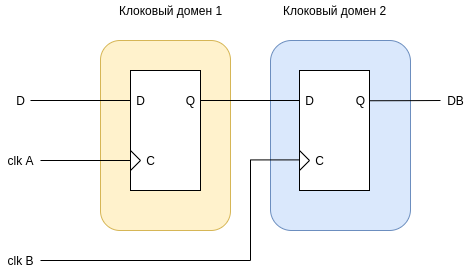
\includegraphics[width=0.7\linewidth]{course-scheme/images/multiclock-domain}
	\caption{Путь домена синхрочастоты}
	\label{fig:multiclock-domain}
\end{figure}


\section{Основные принципы}

При разработке ультисинхрочастотных проектов следует уделять особое внимание стабильности сигнала. Когда сигнал пересекает домен синхрочастоты, то он появляется в новом домене синхрочастоты как асинхронный сигнал и должен быть засинхронизирован.

Синхронизация предотвращает в новом домене синхрочастоты метастабильное состояние первого запоминающего элемента схемы (триггера), и это позволяет в новом домене работать уже со стабильным сигналом.

\textit{Метастабильность} --- это неспособность триггера достигнуть известного состояния в определенный момент времени. Когда триггер входит в метастабильное состояние, то невозможно предсказать ни уровень выходного напряжения элемента, ни период времени, за который этот выход перейдет к правильному уровню напряжения. 

В течение этого переходного времени выход триггера будет находиться на некотором промежуточном уровне напряжения или колебаться и может передать этот недопустимый уровень сигнала со своего выхода к другим триггерам схемы.

\section{Решение проблемы метастабильности}

С целью решения проблемы метастабильности применяются каскады стабилизирующих триггеров, включенных последовательно. Рассмотрим это решение.


Простейший синхронизатор представляет собой два триггера, включенных последовательно без какой-либо комбинационной схемы между ними. Такая схема проекта гарантирует, что первый триггер выходит из своего метастабильного состояния, и его выход переходит в устойчивое состояние перед тем, как второй триггер сохраняет его. Необходимо также разместить эти триггеры, насколько возможно, ближе друг к другу для того, чтобы гарантировать наименьшую расфазировку тактовых сигналов между ними. 

Другой тип ячейки синхронизатора представляет собой два близко расположенных триггера без какой-либо комбинационной логики между ними. Для того чтобы синхронизация работала должным образом, сигнал, пересекающий домен синхрочастоты, должен проследовать от триггера в домене синхрочастоты источника сигнала к первому триггеру синхронизатора, не пройдя через комбинационную логику.

Синхронизацию в домене называют привязкой входного сигнала к тактовой частоте
домена, т. е. все изменения этого сигнала в домене будут происходить по фронту или срезу
тактового сигнала домена, а не родительского тактового сигнала. На Рисунке \ref{fig:sync-triggers}) приведена схема традиционного синхронизатора из
двух триггеров (сдвиговый регистр) для одиночного сигнала. Схема синхронизации приведена на Рисунке \ref {fig:sync-scheme}.

\begin{figure}[h!]
	\centering
	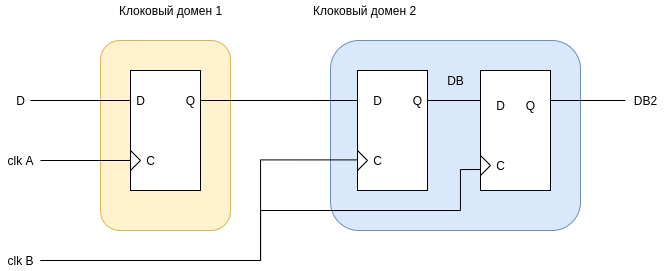
\includegraphics[width=0.6\linewidth]{course-scheme/images/sync-triggers}
	\caption{Триггеры синхронизации}
	\label{fig:sync-triggers}
\end{figure}

\begin{figure}[h!]
	\centering
	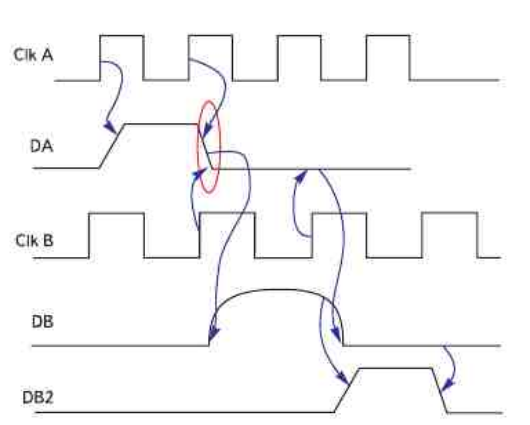
\includegraphics[width=0.3\linewidth]{course-scheme/images/sync-scheme}
	\caption{Схема синхронизации сигнала}
	\label{fig:sync-scheme}
\end{figure}
%\clearpage
%\vspace{2ex}

Данный способ борьбы с метастабильностью будет в дальнейшем использован при разработке узла ресихронизации данных.

\section{Асинхронная очередь}

Во многих проектах необходимо передавать из одного домена в другой не только несколько одиночных сигналов, но и сигналы типа шин: шины данных, адреса и шины управления.

В этих задачах активно используются буферы типа FIFO и специальные протоколы для процедуры установления связи. Особенно полезной оказывается асинхронная очередь, позволяющая производить запись и чтение по синхросигналам двух клоковых доменов.
Данная схема позволяет быстро и удобно передавать данные в реальном времени между двумя разными областями синхронизации.

На Рисунке \ref{fig:async-fifo} приведена схема использования двухпорторой оперативной памяти, позволяющей осуществлять передачу данных между частями устройства, использующими синхросигналы разной частоты.

\begin{figure}[h!]
	\centering
	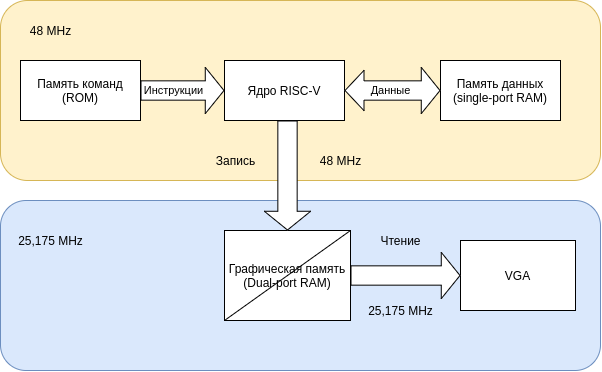
\includegraphics[width=0.65\linewidth]{course-scheme/images/dual-port-ram}
	\caption{Двухпортовая оперативная память}
	\label{fig:async-fifo}
\end{figure}

Двухпортовая память с независимыми тактовыми сигналами --- аппаратный блок, используемый в современных FPGA и в технологических библиотеках для заказных микросхем. Чтение и запись производится совершенно независимо через два отдельных порта.

Единственным ограничением является одновременное обращение на запись и чтение по одному и тому же адресу памяти --- оно может привести к неопределенному результату. На основе такого блока памяти зачастую создается модуль FIFO, который позволяет с одной стороны записывать данные из одного тактового домена, а с другой — забирать в другой тактовый домен. Заодно логика FIFO следит за тем, чтобы не происходило обращения к одной и той же ячейке памяти.

Данный узел работает по следующему принципу. 
\begin{enumerate}
	\item Источник данных загружает данные в асинхронную очередь. Тактирование производится по тактовому сигналу источника данных.
	\item Потребитель данных считывает данные из асинхронной очереди в исходном порядке. Тактирование производится по тактовому сигналу потребителя данных. 
\end{enumerate}




\clearpage
\newcommand{\erdatamodaler}{ERwin Data Modeler~}

\chapter{Создание логической и физической модели данных}
\label{cha:dmd}
В данном разделе будет рассмотрено создание логической и физической модели данных предложенных предметных областей в ПО ERwin Data Modeler.

На этапе инфологического проектирования базы данных должна быть построена
модель предметной области, не привязанная к конкретной СУБД, понятная не только
разработчикам информационной системы, но и экономистам, менеджерам и другим
специалистам. В то же время модель предметной области должна максимально точно
отражать семантику предметной области и позволять легко перейти к модели данных
конкретной СУБД.

\textbf{Логический уровень} --- это уровень, соответствующий инфологическому этапу проектирования
и не привязанный к конкретной СУБД. Модели логического уровня оперируют с
понятиями сущностей, атрибутов и связей, которые на этом уровне именуются на
естественном языке (в нашем случае – на русском) так, как они называются в
реальном мире.

\textbf{Физический уровень} --- это отображение логической модели на модель данных
конкретной СУБД. Одной логической модели может соответствовать несколько
физических моделей. Причем, Erwin (как и другие CASE-системы проектирования баз
данных) позволяет автоматизировать отображение логической модели на физическую.

\section{Работа по методическим указаниям}

Порядок построения модели данных в среде \erdatamodaler рассмотрим на примере
автоматизированной информационной системы <<Реализация средств вычислительной
техники>>, предназначенной для учета продаж настольных компьютеров по заказам
клиентов.

Создание модели данных начинается с разработки логической модели, которая
должна представлять состав сущностей предметной области с перечнем атрибутов и
отношений между ними.

Результат разработки логической модели данных системы <<Реализация средств
вычислительной техники>>, предназначенной для учета продаж настольных
компьютеров по заказам клиентов приведен на Рисунке \ref{fig:2-logical-model-method}.

% TODO: \usepackage{graphicx} required
\begin{figure}[htpb]
	\centering
	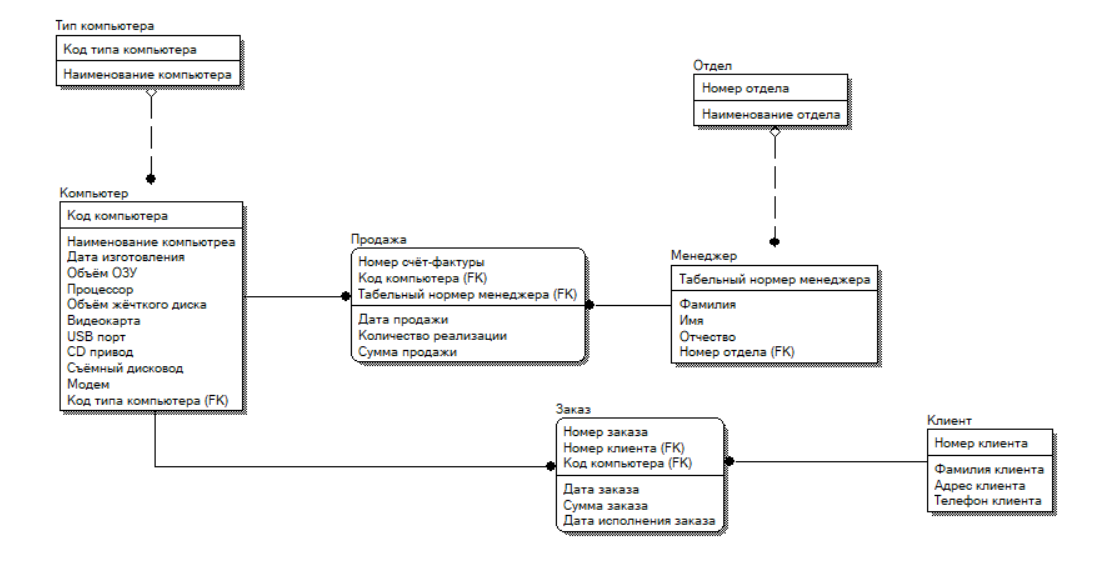
\includegraphics[angle=0,width=\linewidth]{/2-method}
	\caption{Логическая модель данных системы <<Реализация средств вычислительной техники>>}
	\label{fig:2-logical-model-method}
\end{figure}

Для построения физической модели данных системы, следует определиться с СУБД, в которой будет реализована модель. При построении физической модели данных следует учитывать формальную теория представления и обработки данных в конкретной системе управления базами данных (СУБД).

В данной практической работе в качестве СУБД выбрана MySQL.

Приступим к построению физической модели данных системы <<Реализация средств вычислительной техники>>. Результат работы можно видеть на Рисунке \ref{fig:2-phisical-model}.
%\newpage
% TODO: \usepackage{graphicx} required
\begin{figure}[ht]
	\centering
	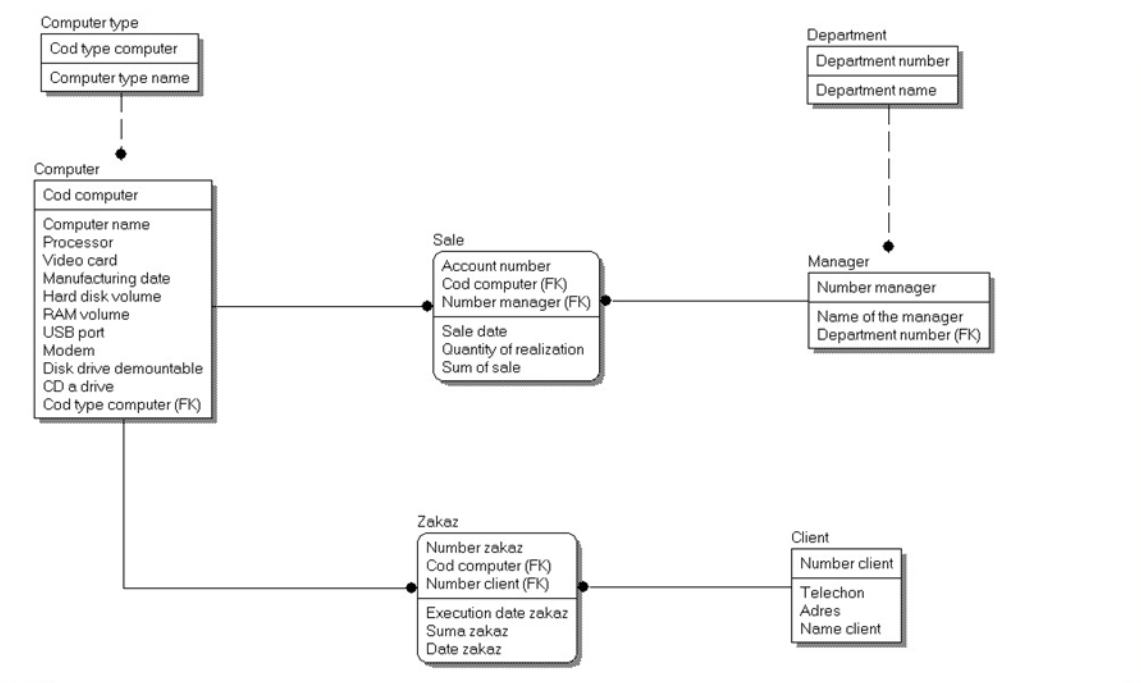
\includegraphics[angle=0,width=\linewidth]{2-phisical-model}
	\caption{Физическая модель данных системы <<Реализация средств вычислительной техники>>}
	\label{fig:2-phisical-model}
\end{figure}
\newpage
\subsection{Индивидуальное задание}
Приступим к построению логической модели данных системы <<Велосипедное предприятие>>. 
В соответствии с моделью, реализованной в ходе первой практической работы, добавим в рабочую область следующие сущности:
\begin{itemize}
	\item Component;
	\item FrameInfo;
	\item Frame;
	\item Frameset;
	\item FrameSize;
	\item Fork;
	\item ComponentType;
	\item Wheelset;
	\item Groupset;
	\item Brake;
	\item FctCycleBuild;
	\item CycleType;
	\item Bar;
	\item Setup.
\end{itemize}
Добавим связи между сущностями в соответствии с ранее построенной моделью. Логическая модель системы <<Велосипедное предприятие>> приведена на Рисунке \ref{fig:2-cycle-logical}.

% TODO: \usepackage{graphicx} required
\begin{figure}[h!]
	\centering
	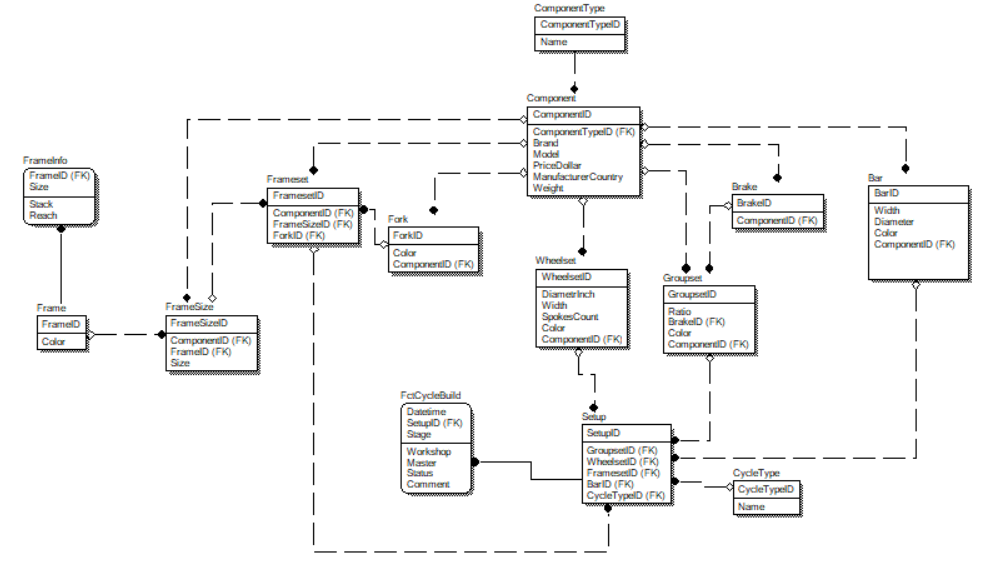
\includegraphics[width=0.8\linewidth]{2-cycle-logical}
	\caption{Логическая модель данных системы <<Велосипедное предприятие>>}
	\label{fig:2-cycle-logical}
\end{figure}

После уточнения типов данных, выбранных в соответствии с предметной областью и спецификой СУБД MySQL.
Физическая модель системы <<Велосипедное предприятие>> приведена на Рисунке \ref{fig:2-cycle-phisical}.

% TODO: \usepackage{graphicx} required
\begin{figure}[h!]
	\centering
	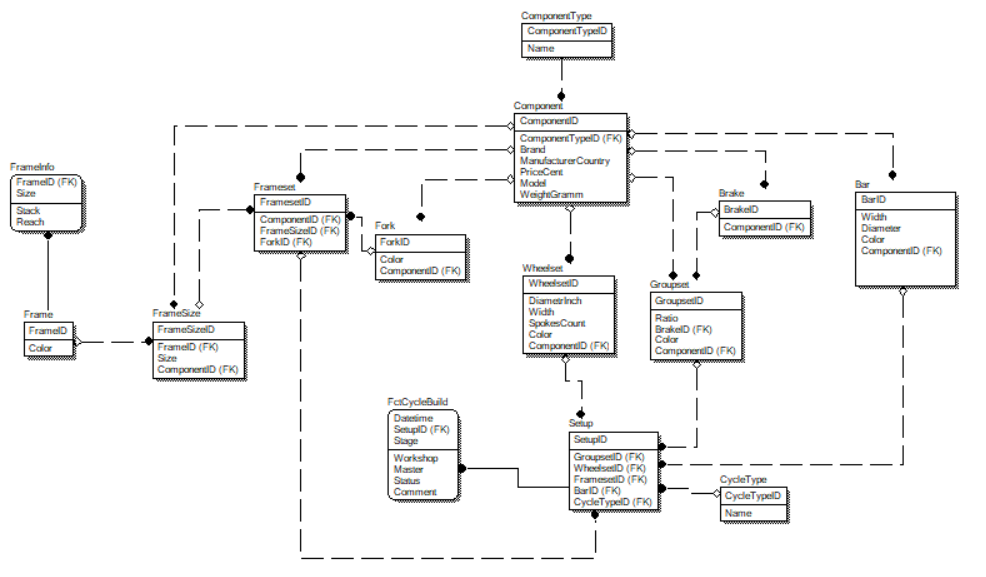
\includegraphics[width=0.8\linewidth]{2-cycle-phisical}
	\caption{Физическая модель данных системы <<Велосипедное предприятие>>}
	\label{fig:2-cycle-phisical}
\end{figure}

После реализации физической и логической модели можно приступать к реализации модели данной системы в СУБД MySQL.
\hfill
\clearpage
\chapter{Создание базы данных}
\section{Работа по методическим указаниям}
Создадим базу данных \texttt{forum}, которая хранит в себе сведения о пользователях форумах и размещенных ими темах.

Помимо суперпользователя root, был создан пользователь denilai, под которым производятся все манипуляции с данными.

Создадим базу данных \texttt{forum} с помощью команды \texttt{CREATE DATABASE forum;}


Создадим таблицу \texttt{users} (см. Рисунок \ref{fig:create-users}):

% TODO: \usepackage{graphicx} required
\begin{figure}[h!]
	\centering
	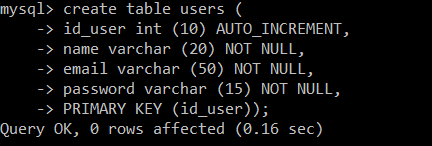
\includegraphics[width=0.7\linewidth]{create-users}
	\caption{Создание базы данных users}
	\label{fig:create-users}
\end{figure}

%\begin{lstlisting}
%create table users (
%	id_user INT (10) AUTO_INCREMENT,
%	name varchar(20) NOT NULL,
%	email varchar(50) NOT NULL,
%	password varchar(15) NOT NULL,
%	PRIMARY KEY (id_user)
%);
%\end{lstlisting}

Создадим таблицу \texttt{topics} (см. Рисунок \ref{fig:create-topics}):

% TODO: \usepackage{graphicx} required
\begin{figure}[h!]
	\centering
	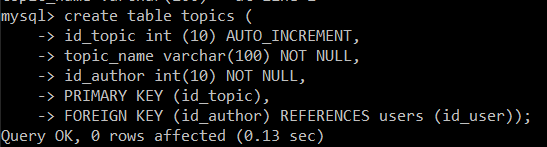
\includegraphics[width=0.7\linewidth]{create-topics}
	\caption{Создание базы данных topics}
	\label{fig:create-topics}
\end{figure}

%\begin{lstlisting}
%create table topics (
%	id_topic INT (10) AUTO_INCREMENT,
%	topic_name varchar(100) NOT NULL,
%	id_author INT (10) NOT NULL,
%	PRIMARY KEY (id_topic),
%	FOREIGN KEY (id_author) REFERENCES users (id_user)
%);
%\end{lstlisting}
Создадим таблицу \texttt{posts} (см. Рисунок \ref{fig:create-posts}):

\begin{figure}[h!]
	\centering
	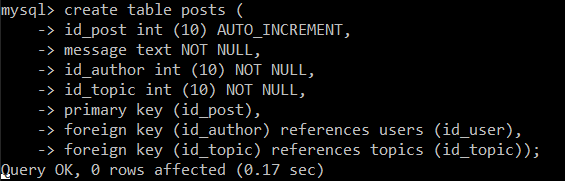
\includegraphics[width=0.7\linewidth]{create-posts}
	\caption{Создание базы данных posts}
	\label{fig:create-posts}
\end{figure}

После создания таблиц, заполним их данными о пользователях форума, о темах и размещенных публикациях. Выполним операцию выборки данных без условия, чтобы увидеть все записи, занесенные в таблицы с помощью команды \texttt{SELECT * FROM <table-name>} (см. Рисунок \ref{fig:select-from-all}). 

% TODO: \usepackage{graphicx} required
\begin{figure}[h!]
	\centering
	\includegraphics[width=0.8\linewidth]{select-from-all}
	\caption{Операция выборки из всех таблиц }
	\label{fig:select-from-all}
\end{figure}

Выполним запрос \texttt{SELECT mesage, topic\_name FROM posts p JOIN topics t ON t.id\_author = p.id\_author; } для объединения данных из таблиц \texttt{topics} и \texttt{posts} по ключу id\_author и получения полной информации о сообщении и названию темы, в которой оно было размещено (см. Рисунок \ref{fig:join-post-author}).

% TODO: \usepackage{graphicx} required
\begin{figure}[ht]
	\centering
	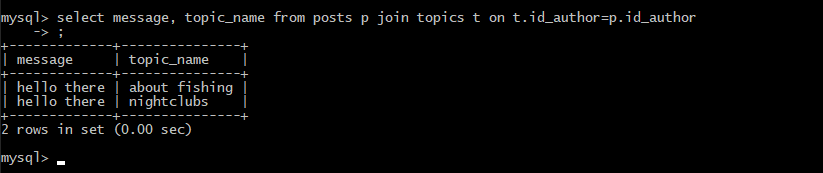
\includegraphics[width=0.8\linewidth]{join-post-author}
	\caption{Запрос объединения}
	\label{fig:join-post-author}
\end{figure}

Выполним запрос выборки данных, явно указав поля отношения. Для этого перечислим имена полей через запятую после зарезервированного слова \texttt{SELECT} (см. Рисунок \ref{fig:field-select}).

% TODO: \usepackage{graphicx} required
\begin{figure}[h!]
	\centering
	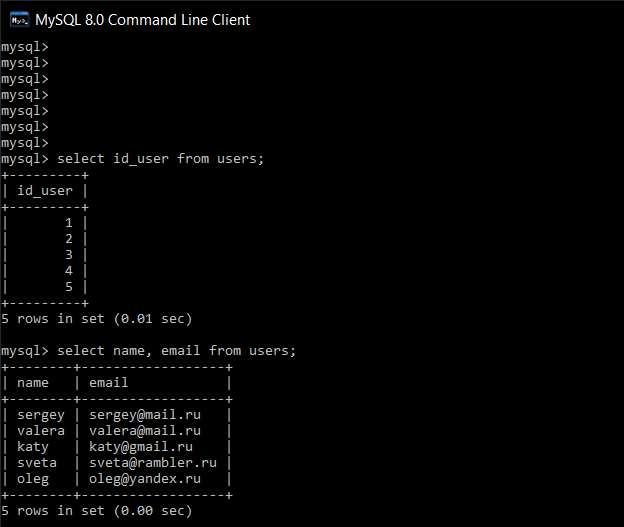
\includegraphics[width=0.5\linewidth]{field-select}
	\caption{Операция выборки с указанием полей}
	\label{fig:field-select}
\end{figure}


Выполним более сложные запросы выборки, отсортировав записи в таблице \texttt{topics} по убыванию значения поля \texttt{topic\_name} и \texttt{id\_author}, а также опишем условие сравнения значения поля \texttt{id\_author} в сецкции \texttt{WHERE}(см. Рисунок \ref{fig:order-where-forum}). 

% TODO: \usepackage{graphicx} required
\begin{figure}[h!]
	\centering
	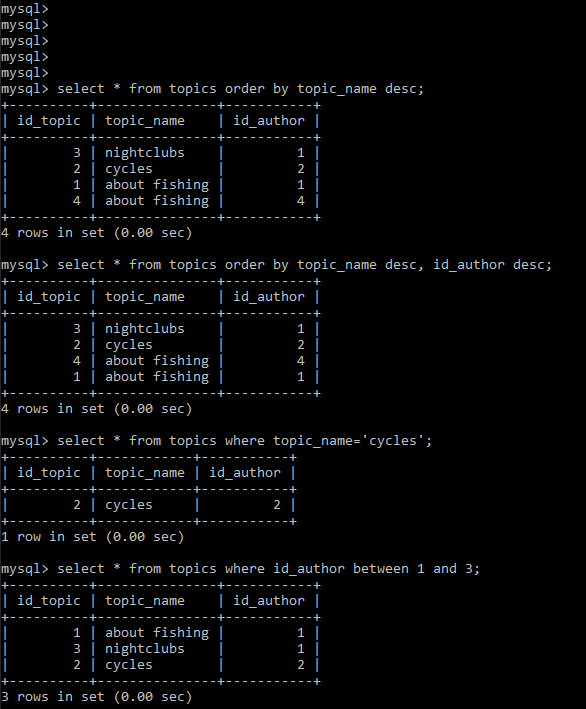
\includegraphics[width=0.5\linewidth]{order-where-forum}
	\caption{Сложные запросы выборки с сортировкой и условием}
	\label{fig:order-where-forum}
\end{figure}

Выполним операции по модификации таблицы --- добавим в таблицу \texttt{users} поле \texttt{country} типа \texttt{varchar (20)} со значением по умолчанию "Russia", а также добавим в эту же таблицу поле \texttt{age int(10)} со значением по умолчанию 19. 

Выведем все записи из таблицы \texttt{users}, обнаружим, что столбцы были вставлены успешно (см. Рисунок \ref{fig:alter-add-forum}).

% TODO: \usepackage{graphicx} required
\begin{figure}[h!]
	\centering
	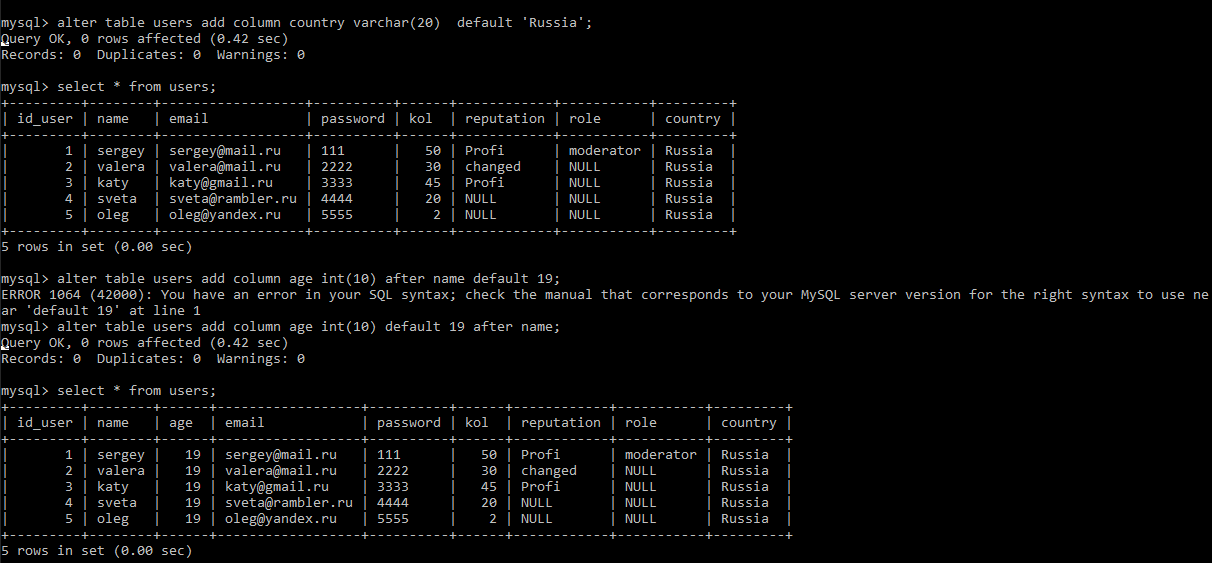
\includegraphics[width=0.9\linewidth]{alter-add-forum}
	\caption{Добавление полей в таблицу \texttt{users}}
	\label{fig:alter-add-forum}
\end{figure}

В ходе данной практической работы были рассмотрены операторы DDL и DML диалекта MySQL. С помощью данных операторов была создана база учебная база данных \texttt{forum}, содержащая о пользователях форумах и размещенных ими темах.

\section{Индивидуальное задание}

Продолжим работу над созданием модели данных велосипедного предприятия. Создадим базу данных \texttt{cycle}, сущностями  которой будут таблицы, описания которых были проработаны в прошлых практических работах. 

Описание проектируемых отношений базы данных \texttt{cycle} приведены в таблицах \ref{tab:bar}--\ref{tab:log}.

%(\textbf{Bar})
\begin{table}[h!] 
	\centering
	\caption{Описание таблицы Bar}
	\begin{tabular}{|l|l|}
		\hline \textbf{Имя} & \textbf{Тип} \\
		\hline
		Width & INTEGER NOT NULL \\ \hline
		Diameter & INTEGER NOT NULL \\ \hline
		BarID & INTEGER NOT NULL AUTO\_INCREMENT \\ \hline
		Color & VARCHAR(20) NULL DEFAULT 'black' \\ \hline
	\end{tabular}
	\label{tab:bar}
\end{table}

%(\textbf{Brake})
\begin{table}[h!] 
	\centering
	\caption{Описание таблицы Brake}
	\begin{tabular}{|l|l|}
		\hline \textbf{Имя} & \textbf{Тип} \\
		\hline
		BrakeID &       INT NOT NULL AUTO\_INCREMENT \\ \hline
		ComponentID &   INTEGER NULL \\ \hline
	\end{tabular}
	\label{tab:brake}
\end{table}


%(\textbf{Component})

\begin{table}[h!] 
	\centering
	\caption{Описание таблицы Component}
	\begin{tabular}{|l|l|}
		\hline \textbf{Имя} & \textbf{Тип} \\
		\hline
		ComponentID &   INTEGER NOT NULL AUTO\_INCREMENT \\ \hline
		Brand & VARCHAR(20) NOT NULL \\ \hline
		ManufacturerCountry &  VARCHAR(20) NOT NULL \\ \hline
		PriceCent & INTEGER NOT NULL \\ \hline
		Model & VARCHAR(20) NOT NULL \\ \hline
		ComponentTypeID &  INTEGER NOT NULL \\ \hline
		WeightGramm &   INTEGER NOT NULL \\ \hline
	\end{tabular}
	\label{tab:component}
\end{table}

%(\textbf{ComponentType}) 
\begin{table}[h!] 
	\centering
	\caption{Описание таблицы ComponentType}
	\begin{tabular}{|l|l|}
		\hline \textbf{Имя} & \textbf{Тип} \\
		\hline
		ComponentTypeID &  INTEGER NOT NULL AUTO\_INCREMENT \\ \hline
		Name & VARCHAR(20) \\ \hline
	\end{tabular}
	\label{tab:componenttype}
\end{table}


%(\textbf{CycleType})

\begin{table}[h!] 
	\centering
	\caption{Описание таблицы CycleType}
	\begin{tabular}{|l|l|}
		\hline \textbf{Имя} & \textbf{Тип} \\
		\hline
		CycleTypeID &   INTEGER NOT NULL AUTO\_INCREMENT \\ \hline
		Name &  VARCHAR(20) NOT NULL \\ \hline
	\end{tabular}
	\label{tab:cycletype}
\end{table}

\begin{table}[h!] 
	\centering
	\caption{Описание таблицы FctCycleBuild}
	\begin{tabular}{|l|l|}
		\hline \textbf{Имя} & \textbf{Тип} \\
		\hline
		SetupID &       INTEGER NOT NULL \\ \hline
		Datetime &      DATE NOT NULL \\ \hline
		Stage & INTEGER NOT NULL \\ \hline
		Workshop &      varchar(20) NOT NULL DEFAULT 'main' \\ \hline
		Master &        VARCHAR(20) NOT NULL \\ \hline
		Status &        VARCHAR(20) NOT NULL \\ \hline
		Comment &       VARCHAR(20) NOT NULL \\ \hline
	\end{tabular}
	\label{}
\end{table}

%(\textbf{Fork})

\begin{table}[h!] 
	\centering
	\caption{Описание таблицы Fork}
	\begin{tabular}{|l|l|}
		\hline \textbf{Имя} & \textbf{Тип} \\
		\hline
		ForkID &  INTEGER NOT NULL AUTO\_INCREMENT \\ \hline
		Color & VARCHAR(20) NULL DEFAULT 'black' \\ \hline
		ComponentID &  INTEGER NULL \\ \hline
	\end{tabular}
	\label{ta:fork}
\end{table}


%(\textbf{Frame})

\begin{table}[h!] 
	\centering
	\caption{Описание таблицы Frame}
	\begin{tabular}{|l|l|}
		\hline \textbf{Имя} & \textbf{Тип} \\
		\hline
		FrameID &  INTEGER NOT NULL AUTO\_INCREMENT \\ \hline
		Color & VARCHAR(20) NULL DEFAULT 'black' \\ \hline
	\end{tabular}
	\label{tab:frame}
\end{table}


%(\textbf{FrameInfo})

\begin{table}[h!] 
	\centering
	\caption{Описание таблицы FrameInfo}
	\begin{tabular}{|l|l|}
		\hline \textbf{Имя} & \textbf{Тип} \\
		\hline
		FrameID &       INTEGER NOT NULL \\ \hline
		Size & INTEGER NOT NULL \\ \hline
		Stack & INTEGER NOT NULL \\ \hline
		Reach & INTEGER NOT NULL \\ \hline
	\end{tabular}
	\label{tab:frameinfo}
\end{table}


%(\textbf{Frameset})

\begin{table}[h!] 
	\centering
	\caption{Описание таблицы Frameset}
	\begin{tabular}{|l|l|}
		\hline \textbf{Имя} & \textbf{Тип} \\
		\hline
		FrameSizeID &   INTEGER NOT NULL AUTO\_INCREMENT \\ \hline
		ForkID &        INTEGER NOT NULL \\ \hline
		FramesetID &    INTEGER NOT NULL \\ \hline
		ComponentID &   INTEGER NOT NULL \\ \hline
	\end{tabular}
	\label{tab:frameset}
\end{table}


%(\textbf{FrameSize})

\begin{table}[h!] 
	\centering
	\caption{Описание таблицы FrameSize}
	\begin{tabular}{|l|l|}
		\hline \textbf{Имя} & \textbf{Тип} \\
		\hline
		FrameID &       INTEGER NOT NULL \\ \hline
		Size &  INTEGER NOT NULL \\ \hline
		FrameSizeID &   INTEGER NOT NULL AUTO\_INCREMENT \\ \hline
		ComponentID &   INTEGER NOT NULL \\ \hline
	\end{tabular}
	\label{tab:framesize}
\end{table}


%(%(\textbf{Groupset}))

\begin{table}[h!] 
	\centering
	\caption{Описание таблицы Groupset}
	\begin{tabular}{|l|l|}
		\hline \textbf{Имя} & \textbf{Тип} \\
		\hline
		Ratio & INTEGER NOT NULL \\ \hline
		BrakeID &       CHAR(18) NOT NULL \\ \hline
		GroupsetID &    INTEGER NOT NULL AUTO\_INCREMENT \\ \hline
		Color & VARCHAR(20) NOT NULL \\ \hline
		ComponentID &   INTEGER NOT NULL \\ \hline
	\end{tabular}
	\label{tab:groupset}
\end{table}


%(\textbf{Setup})

\begin{table}[h!] 
	\centering
	\caption{Описание таблицы Setup}
	\begin{tabular}{|l|l|}
		\hline \textbf{Имя} & \textbf{Тип} \\
		\hline
		GroupsetID &    INTEGER NOT NULL \\ \hline
		WheelsetID &    INTEGER NOT NULL \\ \hline
		FramesetID &    INTEGER NOT NULL \\ \hline
		BarID & INTEGER NOT NULL \\ \hline
		CycleTypeID &   INTEGER NOT NULL \\ \hline
		SetupID &       INTEGER NOT NULL AUTO\_INCREMENT \\ \hline
	\end{tabular}
	\label{tab:setup}
\end{table}


%(\textbf{Wheelset})

\begin{table}[h!] 
	\centering
	\caption{Описание таблицы Wheelset}
	\begin{tabular}{|l|l|}
		\hline \textbf{Имя} & \textbf{Тип} \\
		\hline
		DiametrInch &   INTEGER NOT NULL \\ \hline
		Width & INTEGER NOT NULL \\ \hline
		SpokesCount &   INTEGER NULL \\ \hline
		WheelsetID &    INTEGER NOT NULL AUTO\_INCREMENT \\ \hline
		Color & VARCHAR(20) NOT NULL \\ \hline
		ComponentID &   INTEGER NOT NULL \\ \hline
	\end{tabular}
	\label{tab:wheelset}
\end{table}

\begin{table}[h!] 
	\centering
	\caption{Описание таблицы Log}
	\begin{tabular}{|l|l|}
		\hline \textbf{Имя} & \textbf{Тип} \\
		\hline
		ID &   INTEGER NOT NULL AUTO\_INCREMENT \\ \hline
		msg & VARCHAR{100} NOT NULL \\ \hline
		row\_id & INTEGER NOT NULL \\ \hline
	\end{tabular}
	\label{tab:log}
\end{table}



\newpage\hfill\newpage\hfill\newpage

\subsection{Использование MySQL CLI Client}

Создадим данные таблицы с помощью MySQL CLI Client~---~клиента, предоставляющего доступ к СУБД через интерфейс командой строки, использовав ключевое слово \texttt{CREATE TABLE}. После создания таблиц выполним команду \texttt{SHOW TABLES}, выбрав базу данных \texttt{cycle} (см. Рисунок \ref{fig:show-tables-cycle}).

% TODO: \usepackage{graphicx} required
\begin{figure}[h!]
	\centering
	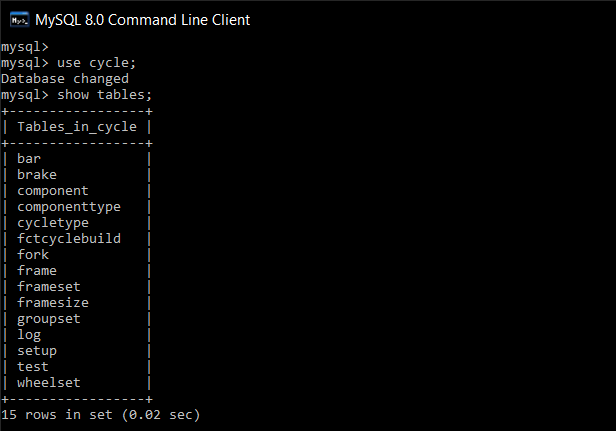
\includegraphics[width=0.5\linewidth]{show-tables-cycle}
	\caption{таблицы базы данных \texttt{cycle}}
	\label{fig:show-tables-cycle}
\end{figure}
Выведем записи из таблицы \texttt{Component} (см. Рисунок \ref{fig:select-components}).

% TODO: \usepackage{graphicx} required
\begin{figure}[h!]
	\centering
	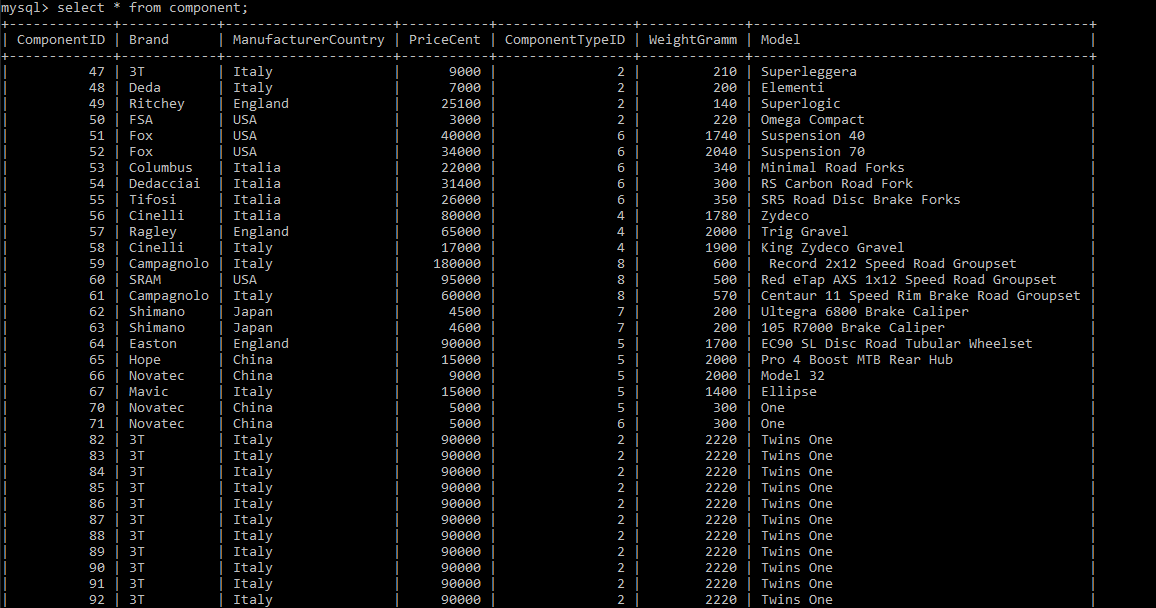
\includegraphics[width=\linewidth]{select-components}
	\caption{Вывод записей из таблицы Components}
	\label{fig:select-components}
\end{figure}

Выполним более сложные запросы выборки --- объединим таблицы с помощью оператора \texttt{INNER JOIN} \texttt{Component} и \texttt{fork} по полю \linebreak \texttt{component\_id}, а также воспользуемся функцией \texttt{ROW\_NUMBER()} в сочетании с оконной функцией \texttt{OVER()}, пронумеровав компоненты из таблицы \texttt{Fork} одного цвета по возрастанию значения поля \texttt{color} (см. Рисунок \ref{fig:join-window-cycle}).

% TODO: \usepackage{graphicx} required
\begin{figure}[h!]
	\centering
	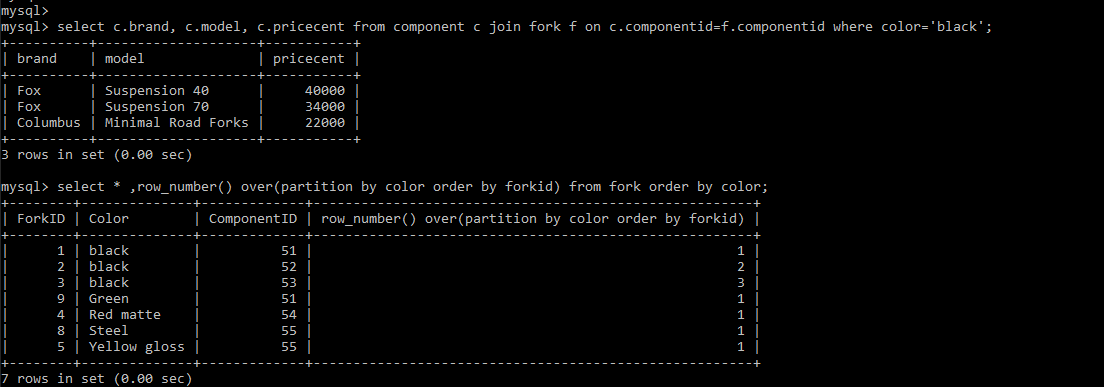
\includegraphics[width=\linewidth]{join-window-cycle}
	\caption{Сложные запросы выборки. База данных cycle}
	\label{fig:join-window-cycle}
\end{figure}


Создадим триггеры \texttt{delete\_component} и  \texttt{add\_component} на добавление и удаление записи в таблице \texttt{Component}. При срабатываении данного триггера, будет добавляться запись в таблицу log, информирующая о совершении манипуляций с данными (см. Листинг \ref{list:trigger}).
%\newpage
Приведем объявление данного триггера на диалекте MySQL:
\lstset{
	language=sql
}
\begin{lstlisting}[caption=Триггер, label={list:trigger}]
DELIMITER $$
drop trigger delete_component; $$

create trigger `delete_component` after delete on component
for each row begin
insert into log (msg, row_id) values (concat('delete component ',old.Brand,' ', old.Model), old.ComponentID);
end; $$

create trigger `add_component` after insert on component
for each row begin
insert into log (msg, row_id) values (concat('insert component ',new.Brand,' ', new.Model), new.ComponentID);
end; $$
DELIMITER $$
\end{lstlisting}

\subsection{Использование MySQL Workbench}

Выполним операции по изменению и просмотру данных, занесенных в базу данных \texttt{cycle}, с помощью инструмента для визуального проектирования баз данных MySQL Workbench.

Для этого подключимся к локально развернутому на машине MySQL Server, указав порт, имя пользователя и пароль. После этого мы получим доступ к пользовательскому интерфейсу программы, представляющему собой две области~---~область выполнения запросов и область отображения результатов (см. Рисунок \ref{fig:workbrench-interface}).

\begin{figure}[h!]
	\centering
	\includegraphics[width=\linewidth]{figures/web-clent/workbrench-interface}
	\caption{Интерфейс MySQL Workbench}
	\label{fig:workbrench-interface}
\end{figure}

Создадим временную таблицу, в котором объединим сведения о компонентах (см. Рисунок \ref{fig:workbrench-components}).
\begin{figure}[h!]
	\centering
	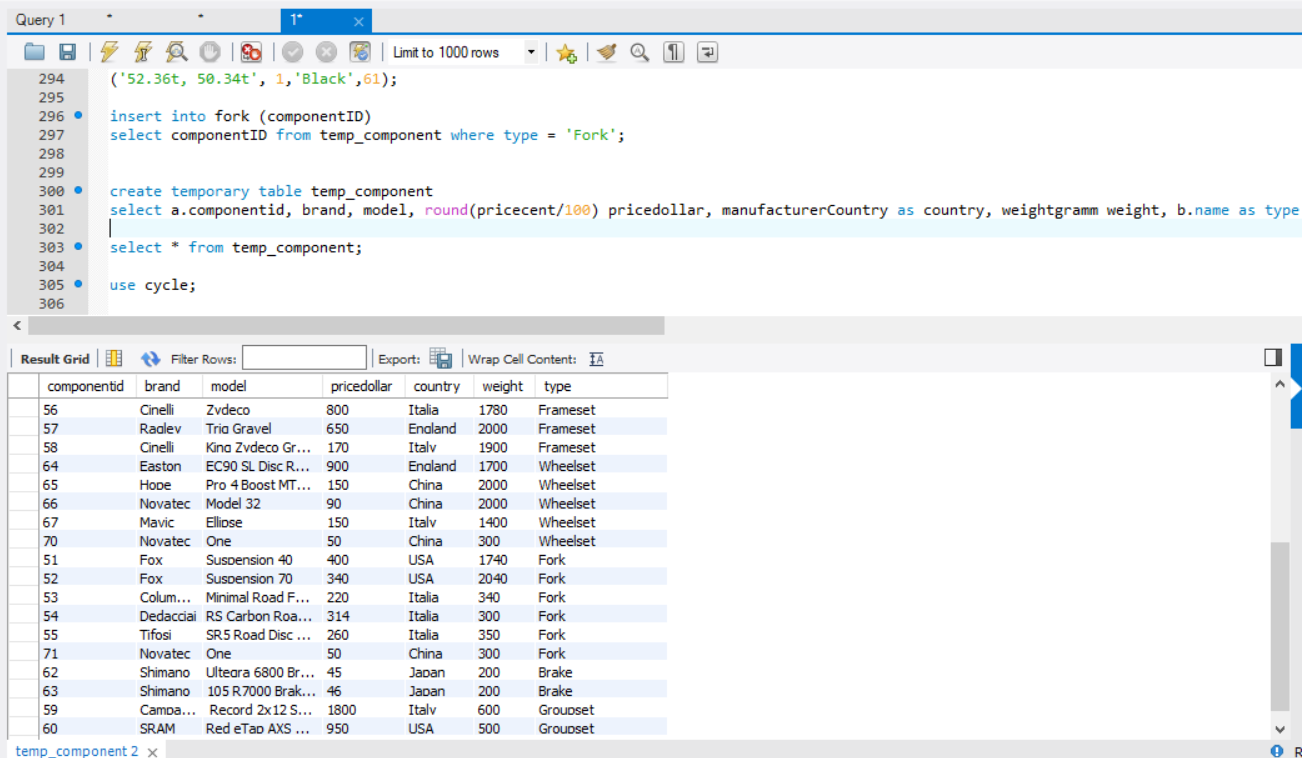
\includegraphics[width=1\linewidth]{figures/web-clent/workbrench-components}
	\caption{Просмотр временной таблицы компонентов}
	\label{fig:workbrench-components}
\end{figure}

Выполним еще один запрос~---~ограничим вывод только компонентами типа <<Fork>> (см. Рисунок \ref{fig:workbrench-forks}).

\begin{figure}[h!]
	\centering
	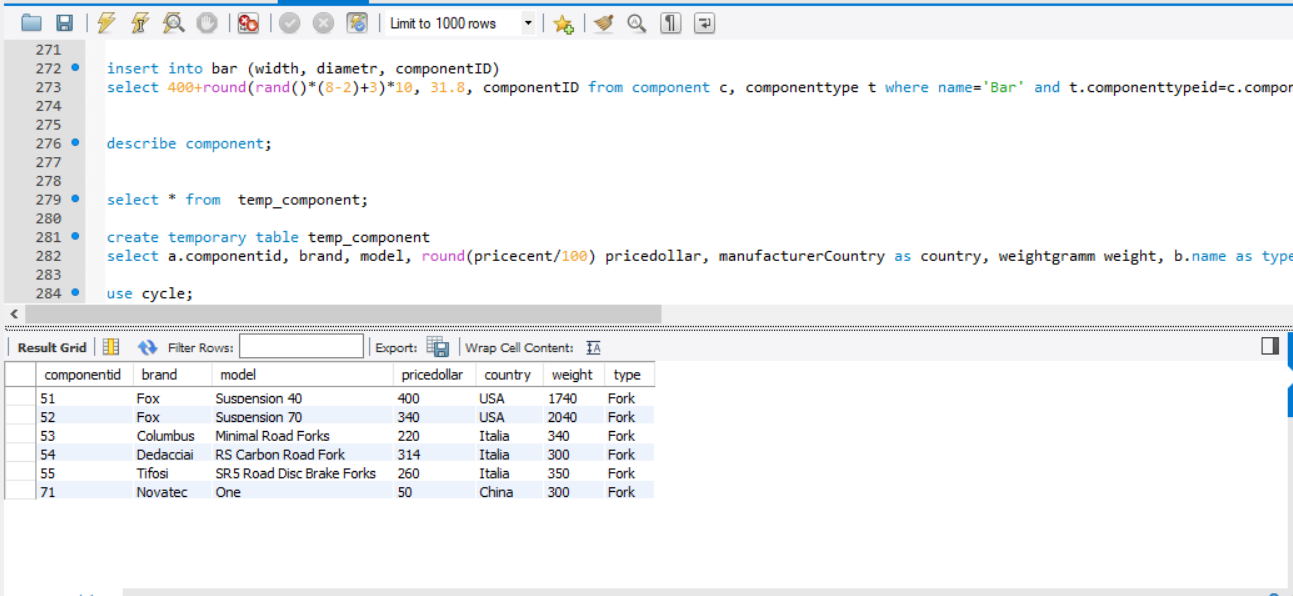
\includegraphics[width=1\linewidth]{figures/web-clent/workbrench-forks}
	\caption{Просмотр временной таблицы компонентов. Компоненты <<Fork>>}
	\label{fig:workbrench-forks}
\end{figure}

Данный визуальный инструмент позволяет удобно организовать работу с базой данных, сохранять SQL--скрипты, параметры подключения и настройки.
\clearpage
\chapter{Создание веб--клиента}

В данном разделе будет рассмотрен процесс реализации веб--приложения, с помощью которого будет производится взаимодействие конечного пользователя с созданной в рамках предыдущих работ базой данных. 

\section{Общие требования к приложению}

Приведем технические требования, предъявляемые к разрабатываемому приложению.

\subsection{Требования к функционалу}
К функционалу приложения предъявляются следующие требования:
\begin{itemize}
	\item регистрация и авторизация пользователя в системе;
	\item добавление, изменение, удаление, обновление информации по
	теме;
	\item фильтрация списков по соответствующим признакам;
	\item просмотр информации по запросу.
\end{itemize}

\subsection{Требования к интерфейсу}

Интерфейс системы должен поддерживать русский язык.

Интерфейс системы должен быть спроектирован с учетом ролевой
модели и уровней доступа пользователей.

Интерфейс системы должен обеспечивать наглядное, интуитивно
понятное представление структуры размещенной информации, быстрый и
логичный переход к соответствующим разделам.

Навигационные элементы интерфейса должны обеспечивать понимание
пользователем их смысла и обеспечивать навигацию по всем доступным
пользователю разделам и отображать соответствующую информацию.

Интерфейс системы должен позволять решать задачи пользователя
наиболее быстрым, простым и удобным из возможных способов.

Дизайн и удобство интерфейса должны быть на уровне ожиданий
современного пользователя и восприниматься им как комфортная, удобная и
приятная рабочая среда.

\section{Реализация приложения}

На основании функциональных требований, указанных в задании, было реализовано веб приложение, позволяющие взаимодействовать с данными, хранящимися в базе данных \texttt{cycle}, созданной в ходе выполнения предыдущих практических работ данного курса.

Интерфейс системы спроектирован с учетом ролевой
модели и уровней доступа пользователей и подразумевает регистрацию пользователя в СУБД MySQL.

Интерфейс поддерживает русский язык и позволяет пользователю удобно просматривать сведения, содержащиеся в таблицах выбранной базы данных.

Акцент в приложении сделан на содержании, дизайн интерфейса прост и лаконичен, чтобы облегчить и упростить взаимодействие пользователя с системой.

\subsection{Используемые технологии}
В качестве набора программных технологий был выбран LAMP--стэк, объединяющий в себе следующие компоненты:
\begin{itemize}
	\item Linux;
	\item Apache;
	\item MySQL;
	\item PHP.
\end{itemize}

Программно-аппаратная часть сервиса (бэкенд) реализована на языке PHP в парадигме объектно-ориентированного программирования, а также с использованием языка MySQL для работы с базой данных.

Структура гипертекстового документа описана средствами HTML и CSS.

Клиентская сторона пользовательского интерфейса системы (фронтэнд) основана на подходе AJAX (Asynchronous Javascript and XML). В качестве языка программирования был использован Java Script. 

Запросы веб-сервиса обрабатываются сервером Apache. 

\subsection{Возможные сценария использования веб-приложения}

Реализуемое веб--приложение может быть использовано для просмотра таблиц, добавления данных в таблицы базы данных под управлением СУБД MySQL, а также для написания произвольных DML и DDL запросов на диалекте MySQL. 

Веб--приложение объединяет в себе часть возможностей командой строки СУБД MySQL и веб-клиента для просмотра таблиц.


\subsection{Демонстрация работы веб-приложения}

Продемонстрируем общие сценарий использования веб--приложения, созданного в рамках данной практической работы. 

\subsubsection{Авторизация}
При первом входе на сайт пользователю необходимо авторизоваться и выбрать пользователя СУБД MySQL, который имеет права на изменение и просмотр данных в выбранной базе данных. Форма авторизации приведена на Рисунке \ref{fig:auth-empty}.
\begin{figure}[h!]
	\centering
	\includegraphics[width=1\linewidth]{figures/web-clent/auth-empty}
	\caption{Авторизация пользователя}
	\label{fig:auth-empty}
\end{figure}


 В данном примере будет выбран пользователь \texttt{denilai}, который имеет привилегии супер-пользователя в данной базе данных и может вносить изменения в базу даннных, просматривать все записи в ней, создавать новые постоянные и временные таблицы, процедуры и макросы.



\subsubsection{Отображение записей таблиц}
После успешной авторизации пользователю будет предложено выбрать таблицу в базе данных, записи в которой будут отображены на экране. Поля таблиц могут содержать кириллические символы --- они будут корректно отображаться веб-приложением (см. Рисунки \ref{fig:select-1}, \ref{fig:select-log}). %\cite{converse2004php5} \cite{baldinLatex} \cite{d2004mysql} \cite{yurt2011dev}

% TODO: \usepackage{graphicx} required
\begin{figure}[h!]
	\centering
	\includegraphics[width=1\linewidth]{web-clent/select-1}
	\caption{Отображение записей таблицы Component}
	\label{fig:select-1}
\end{figure}

% TODO: \usepackage{graphicx} required
\begin{figure}[h!]
	\centering
	\includegraphics[width=1\linewidth]{web-clent/select-1}
	\caption{Отображение записей таблицы Log}
	\label{fig:select-log}
\end{figure}



\subsubsection{Добавление записей в в таблицы}
Ниже, под выведенными записями таблицы расположены поля для добавления значений в выбранную базу данных. В случае ввода корректных данных, после нажатия кнопки <<OK>>, поля будут немедленно добавлены в таблицу и отобразятся на экране (см. Рисунок \ref{fig:insert-1}).

% TODO: \usepackage{graphicx} required
\begin{figure}[h!]
	\centering
	\includegraphics[width=1\linewidth]{web-clent/insert-1}
	\caption{Добавление записей в таблицу Frame}
	\label{fig:insert-1}
\end{figure}


\subsubsection{Выполнение произвольных запросов}
В самом низу веб--страницы расположено текстовое поле для выполнения SQL--запросов. Запросы могут относиться не только к выбранной таблице или базе данных, а к любой таблице, права на взаимодействие с которой имеет выбранный пользователь. 

Текст, введенный пользователем, передается в виде строки на исполнение MySQL серверу. В случае ввода корректного запроса, он будет выполнен, о чем будет сообщено пользователю. 

С помощью данного поля также можно производить операции по удалению и вставке записей в таблицы, отображаемые на экране (см. Рисунок \ref{fig:request}).

% TODO: \usepackage{graphicx} required
\begin{figure}[h!]
	\centering
	\includegraphics[width=1\linewidth]{web-clent/request}
	\caption{Выполнение произвольных запросов}
	\label{fig:request}
\end{figure}

С помощью данного веб--клиента пользователь может просматривать записи, хранящиеся в базе данных, отмечать продвижение деталей по производственным цехам, отражать текущий статус сборки велосипеда, проверять наличие тех или иных компонентов на складе, получать полную информацию о них. Интерфейс отвечает требованиям, выдвинутым в задании: поддерживает русский язык, акцент в приложении сделан на содержании, дизайн интерфейса прост и лаконичен, чтобы упросить взаимодействие пользователя с системой.


%Воспользуемся декартовым произведением таблиц 







%\begin{lstlisting}
%create table posts (
%	id_post int (10) AUTO_INCREMENT,
%	message text NOT NULL,
%	id_author int (10) NOT NULL,
%	id_topic int (10) NOT NULL,
%	PRIMARY KEY (id_post),
%	FOREIGN KEY (id_author) REFERENCES users (id_user),
%	FOREIGN KEY (id_topic) REFERENCES topics (id_topic)
%);
%\end{lstlisting}

%\cite{d2004mysql},\cite{baldinLatex}, \cite{converse2004php5}, \cite{yurt2011dev}.

\backmatter %% Здесь заканчивается нумерованная часть документа и начинаются ссылки и
            %% заключение

\Conclusion % заключение к отчёту

Результатом работы над данной курсовой работой является ознакомление с проблематикой разработки мультисинхронных устройств, реализация цифрового устройства ресинхронизации данных, представляющего собой асинхронную очередь данных, тактируемого двумя независимыми синхросигналами.

В ходе данной работы были проведены мероприятия по разработке функциональной и структурной схемы цифрового устройства и устройств, необходимых для его работы; созданию модуля, реализующего устройство ресинхронизации данных на языке описания аппаратуры Verilog; включению данного устройства в состав сложных устройств и проведение его отладки и тестирования.

Цели и задачи по реализации устройства для ресинхронизации данных выполнены. 

%%% Local Variables: 
%%% mode: latex
%%% TeX-master: "rpz"
%%% End: 


% % Список литературы при помощи BibTeX
% Юзать так:
%
% pdflatex rpz
% bibtex rpz
% pdflatex rpz

\bibliographystyle{gost780u}
\bibliography{course-scheme/rpz}

%%% Local Variables: 
%%% mode: latex
%%% TeX-master: "rpz"
%%% End: 


\appendix   % Тут идут приложения
%
%\chapter{Картинки}
\label{cha:appendix1}

\begin{figure}
\centering
\caption{Картинка в приложении. Страшная и ужасная.}
\end{figure}

%%% Local Variables: 
%%% mode: latex
%%% TeX-master: "rpz"
%%% End: 

%\chapter{Еще картинки}
\label{cha:appendix2}

\begin{figure}
\centering
\caption{Еще одна картинка, ничем не лучше предыдущей. Но надо же как-то заполнить место.}
\end{figure}

%%% Local Variables: 
%%% mode: latex
%%% TeX-master: "rpz"
%%% End: 


\end{document}

%%% Local Variables:
%%% mode: latex
%%% TeX-master: t
%%% End:
